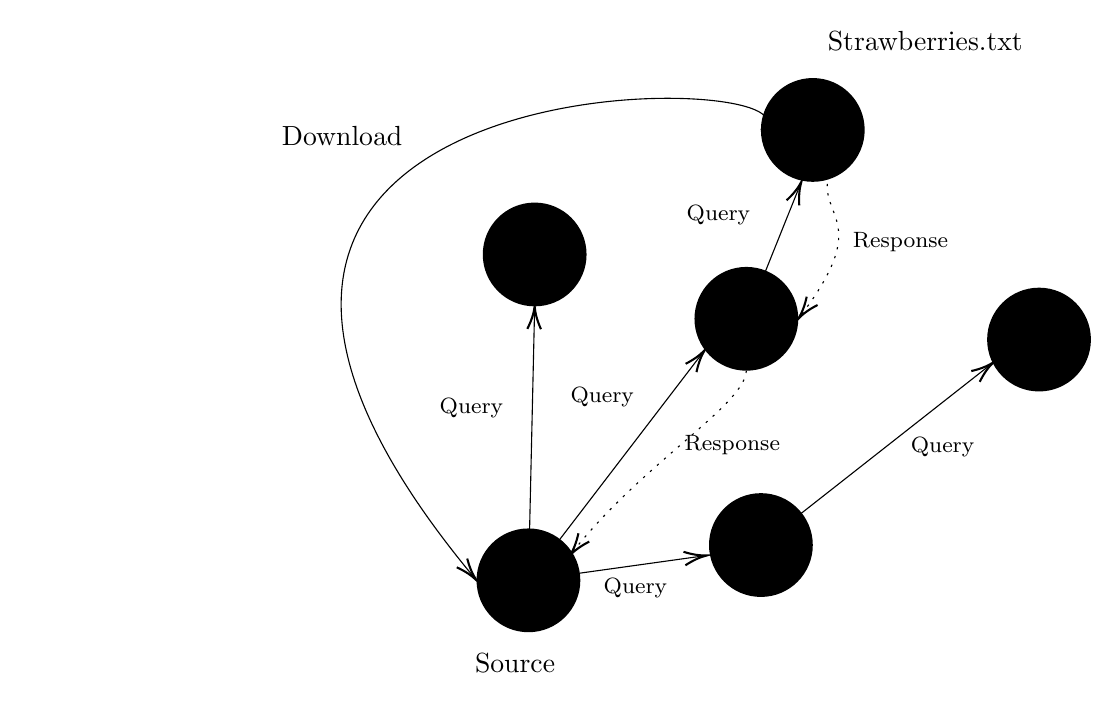
\begin{tikzpicture}[x=0.75pt,y=0.75pt,yscale=-1,xscale=1]
%uncomment if require: \path (0,451); %set diagram left start at 0, and has height of 451

%Shape: Circle [id:dp5701216218873355] 
\draw  [draw opacity=0][fill={rgb, 255:red, 0; green, 0; blue, 0 }  ,fill opacity=1 ] (100,126) .. controls (100,112.19) and (111.19,101) .. (125,101) .. controls (138.81,101) and (150,112.19) .. (150,126) .. controls (150,139.81) and (138.81,151) .. (125,151) .. controls (111.19,151) and (100,139.81) .. (100,126) -- cycle ;
%Shape: Circle [id:dp6701758191642804] 
\draw  [draw opacity=0][fill={rgb, 255:red, 0; green, 0; blue, 0 }  ,fill opacity=1 ] (202,157) .. controls (202,143.19) and (213.19,132) .. (227,132) .. controls (240.81,132) and (252,143.19) .. (252,157) .. controls (252,170.81) and (240.81,182) .. (227,182) .. controls (213.19,182) and (202,170.81) .. (202,157) -- cycle ;
%Shape: Circle [id:dp06164798754338219] 
\draw  [draw opacity=0][fill={rgb, 255:red, 0; green, 0; blue, 0 }  ,fill opacity=1 ] (209,266) .. controls (209,252.19) and (220.19,241) .. (234,241) .. controls (247.81,241) and (259,252.19) .. (259,266) .. controls (259,279.81) and (247.81,291) .. (234,291) .. controls (220.19,291) and (209,279.81) .. (209,266) -- cycle ;
%Shape: Circle [id:dp8491121482645921] 
\draw  [draw opacity=0][fill={rgb, 255:red, 0; green, 0; blue, 0 }  ,fill opacity=1 ] (97,283) .. controls (97,269.19) and (108.19,258) .. (122,258) .. controls (135.81,258) and (147,269.19) .. (147,283) .. controls (147,296.81) and (135.81,308) .. (122,308) .. controls (108.19,308) and (97,296.81) .. (97,283) -- cycle ;
%Shape: Circle [id:dp21625012916250363] 
\draw  [draw opacity=0][fill={rgb, 255:red, 0; green, 0; blue, 0 }  ,fill opacity=1 ] (343,167) .. controls (343,153.19) and (354.19,142) .. (368,142) .. controls (381.81,142) and (393,153.19) .. (393,167) .. controls (393,180.81) and (381.81,192) .. (368,192) .. controls (354.19,192) and (343,180.81) .. (343,167) -- cycle ;
%Shape: Circle [id:dp13339461282709586] 
\draw  [draw opacity=0][fill={rgb, 255:red, 0; green, 0; blue, 0 }  ,fill opacity=1 ] (234,66) .. controls (234,52.19) and (245.19,41) .. (259,41) .. controls (272.81,41) and (284,52.19) .. (284,66) .. controls (284,79.81) and (272.81,91) .. (259,91) .. controls (245.19,91) and (234,79.81) .. (234,66) -- cycle ;
%Straight Lines [id:da3027711082216963] 
\draw    (122,283) -- (124.95,153) ;
\draw [shift={(125,151)}, rotate = 91.3] [color={rgb, 255:red, 0; green, 0; blue, 0 }  ][line width=0.75]    (10.93,-3.29) .. controls (6.95,-1.4) and (3.31,-0.3) .. (0,0) .. controls (3.31,0.3) and (6.95,1.4) .. (10.93,3.29)   ;
%Straight Lines [id:da7950984523527296] 
\draw    (122,283) -- (205.78,173.59) ;
\draw [shift={(207,172)}, rotate = 127.44] [color={rgb, 255:red, 0; green, 0; blue, 0 }  ][line width=0.75]    (10.93,-3.29) .. controls (6.95,-1.4) and (3.31,-0.3) .. (0,0) .. controls (3.31,0.3) and (6.95,1.4) .. (10.93,3.29)   ;
%Straight Lines [id:da09130077482969812] 
\draw    (227,157) -- (252.75,92.86) ;
\draw [shift={(253.5,91)}, rotate = 111.88] [color={rgb, 255:red, 0; green, 0; blue, 0 }  ][line width=0.75]    (10.93,-3.29) .. controls (6.95,-1.4) and (3.31,-0.3) .. (0,0) .. controls (3.31,0.3) and (6.95,1.4) .. (10.93,3.29)   ;
%Straight Lines [id:da12456388559739229] 
\draw    (122,283) -- (206.02,271.28) ;
\draw [shift={(208,271)}, rotate = 172.06] [color={rgb, 255:red, 0; green, 0; blue, 0 }  ][line width=0.75]    (10.93,-3.29) .. controls (6.95,-1.4) and (3.31,-0.3) .. (0,0) .. controls (3.31,0.3) and (6.95,1.4) .. (10.93,3.29)   ;
%Straight Lines [id:da07990008290925488] 
\draw    (234,266) -- (344.43,179.24) ;
\draw [shift={(346,178)}, rotate = 141.84] [color={rgb, 255:red, 0; green, 0; blue, 0 }  ][line width=0.75]    (10.93,-3.29) .. controls (6.95,-1.4) and (3.31,-0.3) .. (0,0) .. controls (3.31,0.3) and (6.95,1.4) .. (10.93,3.29)   ;
%Curve Lines [id:da429610739418806] 
\draw  [dash pattern={on 0.84pt off 2.51pt}]  (266,92) .. controls (265.01,108.83) and (285.58,112.92) .. (253,155.69) ;
\draw [shift={(252,157)}, rotate = 307.69] [color={rgb, 255:red, 0; green, 0; blue, 0 }  ][line width=0.75]    (10.93,-3.29) .. controls (6.95,-1.4) and (3.31,-0.3) .. (0,0) .. controls (3.31,0.3) and (6.95,1.4) .. (10.93,3.29)   ;
%Curve Lines [id:da06143305048271208] 
\draw  [dash pattern={on 0.84pt off 2.51pt}]  (227,182) .. controls (226.01,198.83) and (177,226.44) .. (143.02,269.68) ;
\draw [shift={(142,271)}, rotate = 307.69] [color={rgb, 255:red, 0; green, 0; blue, 0 }  ][line width=0.75]    (10.93,-3.29) .. controls (6.95,-1.4) and (3.31,-0.3) .. (0,0) .. controls (3.31,0.3) and (6.95,1.4) .. (10.93,3.29)   ;
%Curve Lines [id:da928537814793256] 
\draw    (234,66) .. controls (274,36) and (-119,25) .. (97,283) ;
\draw [shift={(97,283)}, rotate = 230.06] [color={rgb, 255:red, 0; green, 0; blue, 0 }  ][line width=0.75]    (10.93,-3.29) .. controls (6.95,-1.4) and (3.31,-0.3) .. (0,0) .. controls (3.31,0.3) and (6.95,1.4) .. (10.93,3.29)   ;

% Text Node
\draw (265,17) node [anchor=north west][inner sep=0.75pt]   [align=left] {Strawberries.txt};
% Text Node
\draw (78,194) node [anchor=north west][inner sep=0.75pt]   [align=left] {{\footnotesize Query}};
% Text Node
\draw (141,189) node [anchor=north west][inner sep=0.75pt]   [align=left] {{\footnotesize Query}};
% Text Node
\draw (197,101) node [anchor=north west][inner sep=0.75pt]   [align=left] {{\footnotesize Query}};
% Text Node
\draw (305,213) node [anchor=north west][inner sep=0.75pt]   [align=left] {{\footnotesize Query}};
% Text Node
\draw (157,281) node [anchor=north west][inner sep=0.75pt]   [align=left] {{\footnotesize Query}};
% Text Node
\draw (277,114) node [anchor=north west][inner sep=0.75pt]   [align=left] {{\footnotesize Response}};
% Text Node
\draw (196,212) node [anchor=north west][inner sep=0.75pt]   [align=left] {{\footnotesize Response}};
% Text Node
\draw (95,317) node [anchor=north west][inner sep=0.75pt]   [align=left] {Source};
% Text Node
\draw (2,63) node [anchor=north west][inner sep=0.75pt]   [align=left] {Download};


\end{tikzpicture}
